% Основная часть
\section{Аналитическая часть}
\subsection{Редакционное расстояние между двумя строками}

\hspace{1.25cm}
Часто требуется измерить различие или расстояние между двумя строками (например, в эволюционных, структуральных или функциональных исследованиях биологических строк, в хранении текстовых баз данных, в методах проверки правописания). Есть несколько способов формализации понятия расстояния между строками. Одна общая и простая, формализация называется редакционным расстоянием; она основана на преобразовании (или редактировании) одной строки в другую серией операций редактирования, выполняемых над отдельными символами. Разрешенные операции редактирования — это вставка (I - insertion) символа в первую строку, удаление (D - deletion) символа из первой строки и подстановка или замена (substitution или, лучше, R - replace) символа из первой строки символом из второй строки. Обозначим M — “не-операцию“ над правильной буквой (от match).

Строка над алфавитом 1, D, R , М, которая описывает преобразование одной строки в другую, называется редакционным предписанием (предписанием) этих двух строк.

Редакционное расстояние между двумя строками определяется как минимальное число редакционных операций — вставок, удалений и подстановок, необходимое для преобразования первой строки во вторую.

Подчеркнем, что совпадения операциями не являются и не засчитываются.
Редакционное расстояние иногда называют расстоянием Левенштейна по статье В. Левенштейна, где оно рассматривалось, вероятно, впервые.\cite{levenshtein}

\subsection{Выравнивание строк}

\hspace{1.25cm}
Редакционное предписание — это способ представления конкретного преобразования одной строки в другую. Альтернативный (и часто предпочтительный) способ заключается в показе явного выравнивания (alignment) этих двух строк.
(Глобальное) выравнивание двух строк, Sl и S2, получается вставкой пробелов в строки S1 и S2 (возможно, на их концах) и размещением двух получившихся строк друг над другом так, чтобы каждый символ или пробел одной строки оказался напротив одного символа или пробела другой строки.

Термин «глобальный» подчёркивает, что обе строки участвуют в выравнивании полностью.\cite{gasfild}

\subsection{Расстояние Левенштейна}

\hspace{1.25cm}
Расстояние Левенштейна, или редакционное расстояние, — метрика cходства между двумя строковыми последовательностями. Чем больше расстояние, тем более различны строки. По сути, это минимальное число односимвольных преобразований (удаления, вставки или замены), необходимых, чтобы превратить одну последовательность в другую.

Цены операций могут зависеть от вида операции (вставка, удаление, замена) и/или от участвующих в ней символов, отражая разную вероятность мутаций в биологии, разную вероятность разных ошибок при вводе текста и т. д. В общем случае:

\begin{itemize}
\item D(a, b) — цена замены символа a на символ b
\item D($\lambda$, b) — цена вставки символа b
\item D(a, $\lambda$) — цена удаления символа a
\end{itemize}

Необходимо найти последовательность замен, минимизирующую суммарную цену. Расстояние Левенштейна является частным случаем этой задачи при ценах:

\begin{itemize}
\item D(a, а) = 0
\item D(a, b) = 1, при a $\neq$ b
\item D($\lambda$, b) = 1
\item D(a, $\lambda$) = 1
\end{itemize}

Как частный случай, так и задачу для произвольных D, решает алгоритм Вагнера — Фишера, приведённый ниже. Здесь и ниже считается, что все D неотрицательны, и действует неравенство треугольника: замена двух последовательных операций одной не увеличит общую цену (например, замена символа x на y, а потом y на z не лучше, чем сразу x на z).

Например, D(’hello’, ‘hallo’) = 1, так как потребуется провести одну замену ‘e’ на ‘a’.

Алгоритм реализуется по следующей формуле:

\begin{equation}
d(S_1, S_2) = D(M, N), \text{где}\\
D(i, j) = 
\begin{cases}
0,  & \text{i = 0, j = 0} \\
i,  & \text{i > 0, j = 0} \\
j,  & \text{i = 0, j > 0} \\
\min
\begin{cases}
D(i-1, j) + 1 & \text{(удаление)} \\
D(i, j-1) + 1 & \text{(вставка)} \\
D(i-1, j-1) + 1_{\text{если}\,a_i \neq b_j} & \text{(замена)}
\end{cases}  & \text{i > 0, j > 0}
\end{cases}
\label{levenshtein_formula}
\end{equation}
\vspace{0.25cm}

Таким образом, требуется вычислить матрицу расстояний размерностью $len(str_1) * len(str_2)$, следовательно, объем требуемой памяти растет как $O(len(str_1) * len(str_2))$. Иными словами, для двух мегабайтных строк потребуются гигабайты памяти. Фактически в кэше будет хранится почти все матрица редактирований, а она не нужна целиком. Искомая цель – правый нижний элемент.

\begin{figure} [H] % Принудительное размещение изображения
	\centering    
    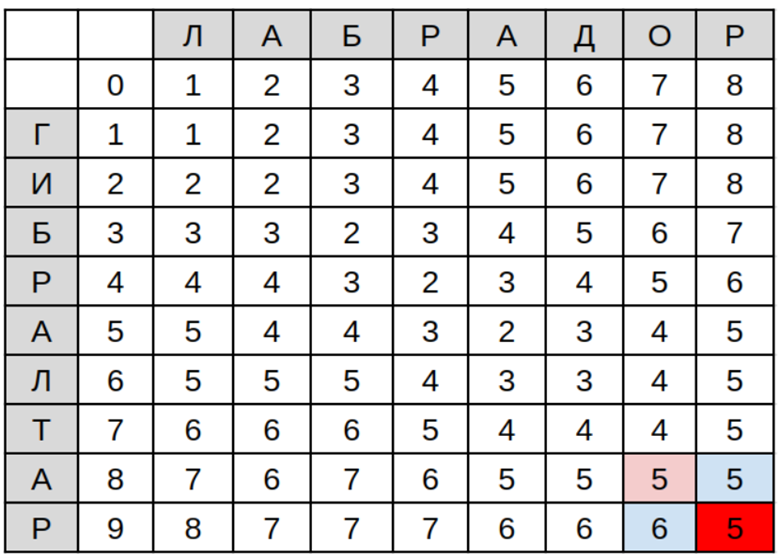
\includegraphics[width=0.9\textwidth]{img/exampleLeven.png} % путь к изображению и размер
    \caption{Пример нахождения расстояния Левенштейна}
\end{figure}

Для его поиска можно обойтись лишь парой рядов: текущим и предыдущим. А остальные ряды не хранить в памяти. Так будет достигнут конец таблицы, и нижний правый угол и будет искомым значением.

Чтобы использовать еще меньше памяти, можно поменять местами строки, чтобы длина рядов была минимальна. Это существенно экономит память, если одна из строк длинная, а другая короткая.

\subsection{Расстояние Дамерау-Левенштейна}

\hspace{1.25cm}
Если к списку разрешённых операций добавить транспозицию (два соседних символа меняются местами), получается расстояние Дамерау — Левенштейна. Для неё также существует алгоритм, требующий O(len(str1) * len(str2)) операций. Дамерау показал, что 80\% ошибок при наборе текста человеком являются транспозициями. Кроме того, расстояние Дамерау-Левенштейна используется и в биоинформатике.

Цена операции транспозиция также равна 1. При работе алгоритма Левенштейна эта операция реализовалась бы двумя заменами и стоила бы 2. Таким образом, расстояние Дамерау-Левенштейна в некоторых случаях даёт меньший результат, чем расстояние Левенштейна.

В формулу \ref{levenshtein_formula} добавляется следующая часть:

\begin{equation}
\begin{cases}
i > 1 \\
j > 1 \\
\text{str}_1[i-1] = \text{str}_2[j] \\
\text{str}_1[i] = \text{str}_2[j-1]
\end{cases}
\label{new_part_formula}
\end{equation}

В результате получается следующая формула для алгоритма Дамерау-Левенштейна:

\begin{equation}
d(S_1, S_2) = D(M, N), \text{где}\\
D(i, j) = 
\begin{cases}
0,  & \text{i = 0, j = 0} \\
i,  & \text{i > 0, j = 0} \\
j,  & \text{i = 0, j > 0} \\
\min
\begin{cases}
D(i-1, j) + 1 & \text{(удаление)} \\
D(i, j-1) + 1 & \text{(вставка)} \\
D(i-1, j-1) + 1_{\text{если}\,a_i \neq b_j} & \text{(замена)} \\
\begin{cases}
i > 1 \\
j > 1 \\
\text{str}_1[i-1] = \text{str}_2[j] \\
\text{str}_1[i] = \text{str}_2[j-1]
\end{cases}  & \text{(транспозиция)}
\end{cases}  & \text{i > 0, j > 0}
\end{cases}
\label{damerau_formula}
\end{equation}

\newpage